\documentclass[12pt,a4paper]{amsart}
\usepackage[slovene]{babel}
%\usepackage[cp1250]{inputenc}
\usepackage[T1]{fontenc}
\usepackage[utf8]{inputenc}
\usepackage{amsmath,amssymb,amsfonts}
\usepackage{url}
\usepackage[normalem]{ulem}
\usepackage[dvipsnames,usenames]{color}
\usepackage{graphicx}

% Oblika strani
\textwidth 15cm
\textheight 24cm
\oddsidemargin.5cm
\evensidemargin.5cm
\topmargin-5mm
\addtolength{\footskip}{10pt}
\pagestyle{plain}
\overfullrule=15pt % oznaci predlogo vrstico


% Ukazi za matematična okolja
\theoremstyle{definition} % tekst napisan pokončno
\newtheorem{definicija}{Definicija}[section]
\newtheorem{primer}[definicija]{Primer}
\newtheorem{opomba}[definicija]{Opomba}

\renewcommand\endprimer{\hfill$\diamondsuit$}


\theoremstyle{plain} % tekst napisan poševno
\newtheorem{lema}[definicija]{Lema}
\newtheorem{izrek}[definicija]{Izrek}
\newtheorem{trditev}[definicija]{Trditev}
\newtheorem{posledica}[definicija]{Posledica}


% Za številske mnozice uporabi naslednje simbole
\newcommand{\R}{\mathbb R}
\newcommand{\N}{\mathbb N}
\newcommand{\Z}{\mathbb Z}
\newcommand{\C}{\mathbb C}
\newcommand{\Q}{\mathbb Q}

% Ukaz za slovarsko geslo
\newlength{\odstavek}
\setlength{\odstavek}{\parindent}
\newcommand{\geslo}[2]{\noindent\textbf{#1}\hspace*{3mm}\hangindent=\parindent\hangafter=1 #2}


\newcommand{\program}{Finančna matematika} 
\newcommand{\imeavtorja}{Neža Kržan} 
\newcommand{\imementorja}{izr. prof. Jaka Smrekar} 
\newcommand{\naslovdela}{Statistika v kazenskem pravu}
\newcommand{\letnica}{2023} %letnica diplome


\begin{document}

%%%%%%%%%%%%%%%%%%%%%%%%%%%%%%%%%%%%%%%%%%%%%%%%%%%%%%%%%%%%%%%%%%%%%%%%%%%%%%%%%%%%%%%%%%%%%%%%%%%%%%%%%%%%%%%%%%%%%%%%%%%%%%%%%%%%%%%%%%%%
\thispagestyle{empty}
\noindent{\large
UNIVERZA V LJUBLJANI\\[1mm]
FAKULTETA ZA MATEMATIKO IN FIZIKO\\[5mm]
\program\ -- 1.~stopnja}
\vfill

\begin{center}{\large
\imeavtorja\\[2mm]
{\bf \naslovdela}\\[10mm]
Delo diplomskega seminarja\\[1cm]
Mentor: \imementorja}
\end{center}
\vfill

\noindent{\large
Ljubljana, \letnica}
\pagebreak

%%%%%%%%%%%%%%%%%%%%%%%%%%%%%%%%%%%%%%%%%%%%%%%%%%%%%%%%%%%%%%%%%%%%%%%%%%%%%%%%%%%%%%%%%%%%%%%%%%%%%%%%%%%%%%%%%%%%%%%%%%%%%%%%%%%%%%%%%%%%
\thispagestyle{empty}
\tableofcontents
\pagebreak

%%%%%%%%%%%%%%%%%%%%%%%%%%%%%%%%%%%%%%%%%%%%%%%%%%%%%%%%%%%%%%%%%%%%%%%%%%%%%%%%%%%%%%%%%%%%%%%%%%%%%%%%%%%%%%%%%%%%%%%%%%%%%%%%%%%%%%%%%%%%
\thispagestyle{empty}
\begin{center}
{\bf \naslovdela}\\[3mm]
{\sc 
V diplomski nalogi se bom osredotočila na statistiko v kazenskem pravu in na zmote, ki se pojavljajo pri uporabi le te, zaradi pomanjkanja
znanja statistike pri odvetnikih, sodnikih in poroti. Osredotočila se bom na uporabo Bayesove statistike v kazenskih postopkih oziroma na izračune,
ki izhajajo iz Bayesove statistike in jo primerjala z drugimi metodami. V nadaljevanju bom opisala in razložila dve najpogostejši zmoti, prva
je Tožilčeva zmota, ki je dobro znan statistični problem, druga večja, ki pa izhaja iz prve, pa je Zmota obrambnega odvetnika. Ker je uporaba
statistike in verjetnostnega računa čedalje pogostejša v sodnih postopkih, bom na koncu pregledala resničen primer sodbe medicinski sestri Lucii de Berk.
}
\end{center}
% tekst povzetka v slovenscini
%V povzetku na kratko opišite vsebinske rezultate dela. Sem ne sodi razlaga organizacije dela -- v katerem poglavju/razdelku je kaj, pač pa le opis vsebine.
\vfill
\begin{center}
{\bf Angleski naslov dela}\\[3mm] % prevod slovenskega naslova dela 
{\sc Abstract}
\end{center}
% tekst povzetka v anglescini
%Prevod zgornjega povzetka v angleščino.

\vfill\noindent
{\bf Math. Subj. Class. (2010):} navedite vsaj eno klasifikacijsko oznako -- dostopne so na \url{www.ams.org/mathscinet/msc/msc2010.html}  \\[1mm]  
{\bf Ključne besede:} navedite nekaj ključnih pojmov, ki nastopajo v delu  \\[1mm]  
{\bf Keywords:} angleški prevod ključnih besed
\pagebreak

%%%%%%%%%%%%%%%%%%%%%%%%%%%%%%%%%%%%%%%%%%%%%%%%%%%%%%%%%%%%%%%%%%%%%%%%%%%%%%%%%%%%%%%%%%%%%%%%%%%%%%%%%%%%%%%%%%%%%%%%%%%%%%%%%%%%%%%%%%%%
%%%%%%%%%%%%%%%%%%%%%%%%%%%%%%%%%%%%%%%%%%%%%%%%%%%%%%%%%%%%%%%%%%%%%%%%%%%%%%%%%%%%%%%%%%%%%%%%%%%%%%%%%%%%%%%%%%%%%%%%%%%%%%%%%%%%%%%%%%%%
%%%%%%%%%%%%%%%%%%%%%%%%%%%%%%%%%%%%%%%%%%%%%%%%%%%%%%%%%%%%%%%%%%%%%%%%%%%%%%%%%%%%%%%%%%%%%%%%%%%%%%%%%%%%%%%%%%%%%%%%%%%%%%%%%%%%%%%%%%%%%%

%%%%%%%%%%%%%%%%%%%%%%%%%%%%%%%%%%%%%%%%%%%%%%%%%%%%%%%%%%%%%%%%%%%%%%%%%%%%%%%%%%%%%%%%%%%%%%%%%%%%%%%%%%%%%%%%%%%%%%%%%%%%%%%%%%%%%%%%%%%%%%





%%%%%%%%%%%%%%%%%%%%%%%%%%%%%%%%%%%%%%%%%%%%%%%%%%%%%%%%%%%%%%%%%%%%%%%%%%%%%%%%%%%%%%%%%%%%%%%%%%%%%%%%%%%%%%%%%%%%%%%%%%%%%%%%%%%%%%%%%%%%%%
%%%%%%%%%%%%%%%%%%%%%%%%%%%%%%%%%%%%%%%%%%%%%%%%%%%%%%%%%%%%%%%%%%%%%%%%%%%%%%%%%%%%%%%%%%%%%%%%%%%%%%%%%%%%%%%%%%%%%%%%%%%%%%%%%%%%%%%%%%%%%%
\section{Bayesova omrežja}
Bayesova omrežja kot taka pomagajo določiti ustrezne verjetnostne formule, ne da bi prikazali njihovo polno algebrsko obliko, in omogočajo
skoraj popolno avtomatizacijo potrebnih verjetnostnih izračunov.
\begin{definicija}
   Bayesovo omrežje(BN) je verjetnostni grafični model, ki predstavlja množico spremenljivk in njihovih pogojnih odvisnosti prek usmerjenega
   acikličnega grafa.
\end{definicija}
Vozlišča teh usmerjenih acikličnih grafov predstavljajo spremenljivke (lahko so opazovane količine, latentne spremenljivke, neznani parametri
ali hipoteze). Povezave predstavljajo pogojne odvisnosti; vozlišča, ki niso povezana, predstavljajo spremenljivke, ki so pogojno neodvisne
druga od druge. Vsako vozlišče je povezano z verjetnostno funkcijo, ki kot vhodni podatek sprejme določen niz vrednosti za nadrejene spremenljivke
vozlišča in kot izhodni podatek poda verjetnost (ali verjetnostno porazdelitev, če je primerno) spremenljivke, ki jo predstavlja vozlišče. Puščice
predstavljajo razmerja pomembnosti, ki jih strokovnjak predvideva v okviru zadevnega problema sklepanja. Usmerjena povezava od vozlišča A do
vozlišča B pomeni, da ima A neposreden vpliv na B. Povezave med vozlišči se včasih razlagajo kot vzročne povezave, vendar opredelitev Bayesovih
omrežij ne zahteva, da povezave predstavljajo vzročni vpliv. Na splošno velja, da povezave v omrežju predstavljajo verjetnostna razmerja
pomembnosti. Značilnost Bayesovih omrežij je vključitev verjetnosti v obliki tabel, povezanih z vsakim vozliščem. To omogoča razlago narave in
moči odnosov med različnimi grafičnimi komponentami omrežja. Tabele verjetnosti vozlišč lahko torej obravnavamo kot sredstvo za povezovanje
modela s podatki.

%%%%%%%%%%%%%%%%%%%%%%%%%%%%%%%%%%%%%%%%%%%%%%%%%%%%%%%%%%%%%%%%%%%%%%%%%%%%%%%%%%%%%%%%%%%%%%%%%%%%%%%%%%%%%%%%%%%%%%%%%%%%%%%%%%%%%%%%%%%%%%
\subsection{Gradnja Bayesovih omrežij}
Obstajajo tri osnovne vrste povezav med vozlišči: zaporedne, razhajajoče se in združevalne povezave. Te so prikazane na sliki 1. \\
\begin{figure}[!ht]\label{fig:slika2}
   \centering
   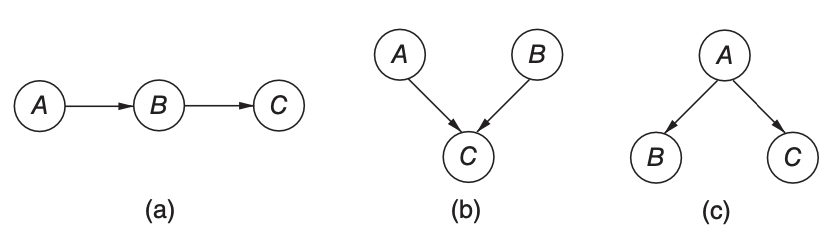
\includegraphics[scale=0.60]{slika4.png}
   \caption{Osnovne povezave v Bayesovih omrežjih:(a)zaporedna, (b)združevalna in (c)razhajajoča povezava.}\vspace{2mm}
\end{figure}
Zaporedna povezava je primerna, kadar presodimo, da poznavanje resničnega stanja $A$ zagotavlja relevantno informacijo o pojavu $B$ in poznavanje
resničnega stanja $B$ posledično zagotavlja relevantno informacijo o $C$, vendar ko je znano resnično stanje $B$, poznavanje stanja $A$ ne
zagotavlja več relevantne informacije o $C$. $A$ vpliva na $C$ preko $B$, vendar samo $B$ neposredno vpliva na $C$. Če je vrednost $B$ znana,
potem sta $A$ in $C$ verjetnostno neodvisna, tj. $P(C \lvert A, B) = P(C \lvert B)$.\\
\textit{Primer zaporedne povezave:\\} naj bodo hipoteze\\
$A \dots$ PoI je storilec kaznivega dejanja;\\
$B \dots$ Krvni madež, najden na kraju kaznivega dejanja, je od PoI;
$c \dots$ Vzorec krvi poškodovanca in krvni madež s kraja kaznivega dejanja imata enak profil DNK. \\
Potem je $A$ relevanten za $B$ in $B$ za $C$, vendar je lahko vzrok za prisotnost krvi glede na $B$ drugačen od $A$.\\\\
Pri združevalni povezavi za tri vozlišča $A$, $B$, $C$ sta $A$ in $B$ verjetnostno neodvisna, razen če je znana vrednost $C$ ali da sta $A$ in $B$
pogojno odvisna glede na vrednost $C$. Tako je $P(AB) = P(A) P(B)$, vendar $P(AB \lvert C) \ne P(A \lvert C) P(B \lvert C)$.\\
\textit{Primer združevalne povezave s tremi vozlišči $A$, $B$, $C$:\\} naj bo\\
$A \dots$ PoI je storilec kaznivega dejanja;\\
$B \dots$ Krvni madež, najden na kraju kaznivega dejanja, je od storilca kaznivega dejanja.\\
Če vemo, da se je eden od teh dogodkov zgodil, ne moremo pridobiti informacij o dogodku drugega, če pa je $C$ (krvni madež, najden na kraju
kaznivega dejanja, izvira od PoI) resničen, potem $A$ in $B$ postaneta povezana.\\\\
Pri razhajajoči se povezavi $A$ ločuje $B$ od $C$. Če je vrednost $A$ znana, potem sta $B$ in $C$ verjetnostno neodvisna, tj.
$P(B \lvert A, C) = P(B \lvert A)$ in $P(C \lvert A, B) = P(C \lvert A)$.

%%%%%%%%%%%%%%%%%%%%%%%%%%%%%%%%%%%%%%%%%%%%%%%%%%%%%%%%%%%%%%%%%%%%%%%%%%%%%%%%%%%%%%%%%%%%%%%%%%%%%%%%%%%%%%%%%%%%%%%%%%%%%%%%%%%%%%%%%%%%%%
\subsection{Uporaba Bayesovih omrežij na sodišču}
Bayesova omrežja, ki temeljijo na Bayesovi teoriji in teoriji grafov, ponujajo forenzičnim znanstvenikom več prefinjenih možnosti. Tem metodam
se daje poseben poudarek, kadar je treba med konkurenčnimi hipotezami izbrati najverjetnejšo, izbira pa mora biti podprta z znanstveno utemeljeno
argumentacijo. Primerna so za analizo dogodka, ki se je zgodil, in napovedovanje verjetnosti, da je k temu prispeval katerikoli od več možnih
znanih vzrokov. Prednosti Bayesovih mrež se najbolj izrazito pokažejo na zapletenih področjih z več spremenljivkami. Kriminalistične aplikacije
Bayesovih omrežij segajo od prepoznavanja storilcev, posameznih in kompleksnih konfiguracij različnih vrst sledi ter problemov sklepanja, ki
vključujejo rezultate analiz DNK.\\
Ti grafični modeli verjetnosti bistveno izboljšajo vrednotenje verjetnostnih razmerij, ki se uporabljajo za ocenjevanje znanstvenih dokazov.
Omogočajo, da se lotimo kompleksnejših verjetnostnih analiz, kot bi bilo to mogoče s tradicionalnimi pristopi. \\\\
Struktura BN v pravnem kontekstu je dovzetna za napačne predpostavke in napake v procesu ustvarjanja. Izbira vozlišč za dokaze je lahko
pristranska glede na to, kakšna vrsta argumenta je predstavljena. Argumenti obrambe ali tožilstva lahko na primer poudarjajo nasprotne sklepe
in zato vključujejo le podskupino dokazov. Če se za izdelavo ne uporablja dosleden okvir, lahko BN, ki jih oblikujejo različne stranke za en
primer, kažejo različne rezultate. Pri oblikovanju BN za pravno sklepanje je ključnega pomena, da se oblikuje omrežje, ki je razumljivo poroti
in sodniku.\\\\
Prikaz BN se mora ujemati z intuitivnim pripisovanjem vzročno-posledičnih povezav med končno hipotezo, kot je "Obtoženec je kriv.", podhipotezo
"Obtoženec je bil na kraju zločina." in dokazi primera. Poleg težav, ki se pojavijo med postopkom strukturiranja, je problematično tudi sklepanje
iz omrežja, če se izvaja ob napačnih predpostavkah. Verjetnosti, tudi če temeljijo na strokovni presoji, so lahko pristranske zaradi dejavnikov
motenj v postopku pridobivanja podatkov. Metode za sklepanje morajo zato zagotoviti, da se verjetnosti omrežij ne razlagajo napačno kot dejstva in
da se izpostavi dejavnik negotovosti. Primerjati morajo verjetnosti za nasprotujoče si hipoteze in morajo zagotoviti okvir za pravnike, da iz
mreže sklepajo na argumente.\\\\

\subsection{Uporaba Bayesovih omrežij na sodišču}
Bayesova omrežja, ki temeljijo na Bayesovi teoriji in teoriji grafov, ponujajo forenzičnim znanstvenikom več prefinjenih možnosti. Tem metodam
se daje poseben poudarek, kadar je treba med konkurenčnimi hipotezami izbrati najverjetnejšo, izbira pa mora biti podprta z znanstveno utemeljeno
argumentacijo. Primerna so za analizo dogodka, ki se je zgodil, in napovedovanje verjetnosti, da je k temu prispeval katerikoli od več možnih
znanih vzrokov. Prednosti Bayesovih mrež se najbolj izrazito pokažejo na zapletenih področjih z več spremenljivkami. Kriminalistične aplikacije
Bayesovih omrežij segajo od prepoznavanja storilcev, posameznih in kompleksnih konfiguracij različnih vrst sledi ter problemov sklepanja, ki
vključujejo rezultate analiz DNK.\\
Ti grafični modeli verjetnosti bistveno izboljšajo vrednotenje verjetnostnih razmerij, ki se uporabljajo za ocenjevanje znanstvenih dokazov.
Omogočajo, da se lotimo kompleksnejših verjetnostnih analiz, kot bi bilo to mogoče s tradicionalnimi pristopi. \\\\
Struktura BN v pravnem kontekstu je dovzetna za napačne predpostavke in napake v procesu ustvarjanja. Izbira vozlišč za dokaze je lahko
pristranska glede na to, kakšna vrsta argumenta je predstavljena. Argumenti obrambe ali tožilstva lahko na primer poudarjajo nasprotne sklepe
in zato vključujejo le podskupino dokazov. Če se za izdelavo ne uporablja dosleden okvir, lahko BN, ki jih oblikujejo različne stranke za en
primer, kažejo različne rezultate. Pri oblikovanju BN za pravno sklepanje je ključnega pomena, da se oblikuje omrežje, ki je razumljivo poroti
in sodniku.\\\\
Prikaz BN se mora ujemati z intuitivnim pripisovanjem vzročno-posledičnih povezav med končno hipotezo, kot je "Obtoženec je kriv.", podhipotezo
"Obtoženec je bil na kraju zločina." in dokazi primera. Poleg težav, ki se pojavijo med postopkom strukturiranja, je problematično tudi sklepanje
iz omrežja, če se izvaja ob napačnih predpostavkah. Verjetnosti, tudi če temeljijo na strokovni presoji, so lahko pristranske zaradi dejavnikov
motenj v postopku pridobivanja podatkov. Metode za sklepanje morajo zato zagotoviti, da se verjetnosti omrežij ne razlagajo napačno kot dejstva in
da se izpostavi dejavnik negotovosti. Primerjati morajo verjetnosti za nasprotujoče si hipoteze in morajo zagotoviti okvir za pravnike, da iz
mreže sklepajo na argumente.\\\\

%%%%%%%%%%%%%%%%%%%%%%%%%%%%%%%%%%%%%%%%%%%%%%%%%%%%%%%%%%%%%%%%%%%%%%%%%%%%%%%%%%%%%%%%%%%%%%%%%%%%%%%%%%%%%%%%%%%%%%%%%%%%%%%%%%%%%%%%%%%%%%
\subsection{Primer uporabe Bayesovega omrežja}





%%%%%%%%%%%%%%%%%%%%%%%%%%%%%%%%%%%%%%%%%%%%%%%%%%%%%%%%%%%%%%%%%%%%%%%%%%%%%%%%%%%%%%%%%%%%%%%%%%%%%%%%%%%%%%%%%%%%%%%%%%%%%%%%%%%%%%%%%%%%%%
%%%%%%%%%%%%%%%%%%%%%%%%%%%%%%%%%%%%%%%%%%%%%%%%%%%%%%%%%%%%%%%%%%%%%%%%%%%%%%%%%%%%%%%%%%%%%%%%%%%%%%%%%%%%%%%%%%%%%%%%%%%%%%%%%%%%%%%%%%%%%%

%%%%%%%%%%%%%%%%%%%%%%%%%%%%%%%%%%%%%%%%%%%%%%%%%%%%%%%%%%%%%%%%%%%%%%%%%%%%%%%%%%%%%%%%%%%%%%%%%%%%%%%%%%%%%%%%%%%%%%%%%%%%%%%%%%%%%%%%%%%
%%%%%%%%%%%%%%%%%%%%%%%%%%%%%%%%%%%%%%%%%%%%%%%%%%%%%%%%%%%%%%%%%%%%%%%%%%%%%%%%%%%%%%%%%%%%%%%%%%%%%%%%%%%%%%%%%%%%%%%%%%%%%%%%%%%%%%%%%%%%
% Seznam uporabljene literature
%https://www.quantstart.com/articles/Bayesian-Statistics-A-Beginners-Guide/
%https://en.wikipedia.org/wiki/Prosecutor%27s_fallacy
%https://www.researchgate.net/publication/267131008_The_interrogator%27s_fallacy
%https://en.wikipedia.org/wiki/Bayesian_network


\end{document}